\chapter{Existující nástroje}

V této kapitole zanalyzujeme některé existující nástroje pro kresbu diagramů a
porovnáme je dle navržených kritérií.

\section{Srovnávací kritéria}

Prvním kritériem pro porovnání nástrojů je jejich kategorie, která vypovídá o
účelu nástroje a cílové skupině zákazníků. Základní kategorie jsou
\begin{itemize}
  \item konceptuální vrstva -- tyto nástroje jsou většinou určené pro tvorbu ER
  diagramů, případně jiným způsobem modelují vztahy a atributy entit, na které
  při datovém modelování vymezujeme svůj diskurz,
  \item logická (též technologická) vrstva -- tyto nástroje umožňují tvorbu
  diagramů s ohledem na typ struktur, v kterých jsou data uchovávána, např.
  relační databáze,
  \item kresba libovolných diagramů -- nástroje, které nejsou omezeny téměř
  žádným standardem či konvencí a umožňují kresbu libovolných diagramů.
\end{itemize}

Dalším kritériem je typ úložiště. Nástroje mohou ukládat svá data do paměti
prohlížeče (lokálně pro uživatele), na své servery, nebo používat externí
úložiště uživatele, například Google Drive. Čím více různých typů úložiště
nástroj podporuje, tím lépe, neboť uživatel může flexibilně zvolit jeho účelům
vyhovující způsob uchovávání dat. Pro živou spolupráci s týmem je lepší sdílené
úložiště a pro lokální práci je vhodnější lokální úložiště.

Kromě uložení rozdělané práce do serializovaného formátu musí nástroj umožnit
export do formátu, který uživatelé využijí pro své účely. Formáty pro export lze
rozdělit do několika kategorií:
\begin{itemize}
  \item serializovaný formát -- většinou se jedná o vlastní formát aplikace a
  takový soubor nelze jinou aplikací otevřít,
  \item rastrové formáty, např. PNG -- mají nejširší využití a podporu, lze je
  použít v dokumentech a na webových stránkách,
  \item vektorové formáty, např. SVG -- nemají tak rozšířenou podporu, nicméně
  jsou vhodnější v dokumentech po estetické stránce (zvlášť při tištění); dále
  existují vektorové editory, pomocí nichž lze výsledek libovolně upravovat bez
  potřeby souboru ve serializovaném formátu; většina webových prohlížečů formát
  SVG podporuje a soubor vykreslí; do této kategorie lze zařadit i jiné otevřené
  strukturované formáty, např. VSDX,
  \item zjednodušený export -- některé nástroje šetří práci uživatele tím, že
  diagram rovnou exportují do HTML, PDF a podobných finálních formátů pro
  okamžitou aplikaci, přestože uživatel může zvolit jiný formát a finální
  vytvořit sám,
  \item schématické formáty, např. SQL -- téměř výhradně u nástrojů logické
  vrstvy; umožňují rovnou vytvářet schémata pro databáze.
\end{itemize}

Stejně jako u typu úložiště, čím více různých formátů exportu nástroj podporuje,
tím lépe, neboť nástroj je flexibilní.

Živá spolupráce je dalším důležitým kritériem. Ve větších týmech a u velkých
projektů je vývoj modelu urychlen, pokud nástroj spolupráci umožňuje.

Posledním, neméně důležitým kritériem, je způsob komercializace. Většina volně
dostupných nástrojů je nějakým způsobem zpoplatněna, ať už se jedná o
jednorázový nebo pravidelný poplatek. Nejčastějším komerčním modelem je verze
zdarma s omezenými funkcemi a dále několik placených plánů různé úrovně s
odemčenými pokročilými funkcemi. U tohoto modelu je důležité vyrovnat funkce
tak, aby byl nástroj použitelný i v bezplatné verzi, a aby byly placené funkce
atraktivní pro uživatele. Při srovnávání budeme věnovat pozornost i tomu, jestli
jsou placené funkce esenciální.

\section{diagrams.net}

Srovnávací kritéria:
\begin{itemize}
  \item kategorie -- kresba libovolných diagramů,
  \item typ úložiště -- lokální, externí, prohlížeč,
  \item export -- serializovaný, rastrový, vektorový, zjednodušený,
  \item živá spolupráce -- částečně podporována (pomocí externích úložišť),
  \item komercializace -- veškeré funkce jsou zdarma a není potřeba uživatelský
  účet; z jiného pohledu lze počítat cenu externích úložišť, ale ta jsou
  volitelná.
\end{itemize}

diagrams.net (dříve draw.io) je obecný open-source kreslící nástroj (který však
nepřijímá změny od ostatních vývojářů) vydaný s licencí Apache License 2.0,
dostupný jako webová aplikace na adrese \url{app.diagrams.net} nebo jako
desktopová aplikace. Desktopová verze aplikace je sestavena stejným způsobem
jako webová, pouze je zabalena pomocí platformy Electron do okna Chromium. Je
vyvinut v běžných we\-bo\-vých tech\-no\-lo\-gi\-ích (Java\-Script, CSS, HTML).

Diagramy lze uložit do serializovaného XML formátu .drawio. V tomto formátu je
pro každý diagram XML element \texttt{diagram}, ve kterém se nachází data
zakódována do Base64. Tato data jsou komprimována pomocí zlib a obsahují další
XML dokument (URL-encoded), tentokrát již serializaci vlastního diagramu. Formát
tak není bez dekomprese čitelný člověkem. Výhodou je, že lze uložit více
diagramů do jednoho souboru a každý pojmenovat. Rozhraní k tomu určené je
identické s listy souboru tabulkových procesorů, jako Microsoft Excel a Google
Sheets.

Soubor s diagramy lze také uložit do formát SVG, který je navíc otevřený a
podporují ho jiné nástroje. Uživatel má při exportu k dispozici možnost
``Include a copy of my diagram'', která do SVG souboru zahrne již zmíněný Base64
řetězec, ve kterém je diagram serializovaný. Ve výsledku to znamená, že takto
exportované SVG soubory umí diagrams.net i otevřít a práce na nich může
plnohodnotně pokračovat. Toto řešení se nám líbí, protože se jedná o schování
vlastního formátu do SVG, který je nejvhodnějším pro přechovávání a zobrazování
diagramů.

Dalšími možnostmi exportu a ukládání jsou
\begin{itemize}
  \item rastrové soubory PNG, JPEG,
  \item soubor PDF, do kterého je ve vektorovém formátu diagram vložen,
  \item soubor HTML, do kterého lze podobně jako v SVG data diagramu uložit v
  serializované formě, případně pouze vložit veřejný odkaz URL na diagram (pokud
  je použito odpovídající úložiště); v tomto souboru je pak zahrnut JavaScript
  od diagrams.net, který diagram vykreslí,
  \item otevřený formát VSDX, původně vyvinutý pro Microsoft Visio.
\end{itemize}

Ze stejných souborů lze diagramy také importovat, ovšem editovat je lze jen
pokud je v nich zahrnut formát drawio, čehož je dosaženo u některých formátů
popsaných výše.

Jako úložiště si lze vybrat Google Drive, OneDrive, Dropbox, GitHub, GitLab,
paměť prohlížeče a místní úložiště (disk uživatele). Soubor lze ze stejných
úložišť i otevřít a importovat, navíc k tomu i z libovolné dostupné URL.

Živá spolupráce je umožněna pouze pokud soubor jako úložiště využívá takové, ke
kterému mají přístup zápisu (popř. pouze čtení) všichni účastnící se uživatelé
(Google Drive, OneDrive, Dropbox, GitHub, GitLab). Tato úložiště je však nutno
manuálně vhodně nastavit (přístup ostatním uživatelům). U všech úložišť je
rychlost reflektování změn ostatních uživatelů podobná -- vcelku pomalá, protože
aplikace musí změny aktivně kontrolovat a načítat.

Menu File $\rightarrow$ Publish chybně napovídá, že se jedná o funkci živé
spolupráce. Ve skutečnosti je uživateli jen zobrazen odkaz na soubor ve vybraném
úložišti (ale pouze pro Google Drive a OneDrive, jinak je tato možnost vypnuta).
Spolupracující uživatel tak musí tento soubor v daném úložišti uložit k sobě
(sdíleně), aby mohla spolupráce začít. 

Jako další možnost jsme zvažovali desktopovou aplikaci s načteným souborem,
který je libovolným externím nástrojem sdílen mezi uživateli. Bohužel, soubor se
nepřenačítá automaticky, ale musí být manuálně synchronizován tlačítkem File
$\rightarrow$ Synchronize (Alt+Shift+S), které je dostupné pouze v desktopové
verzi aplikace. Uživatel je při externí změně souboru upozorněn (avšak ne
spolehlivě vždy) červeným nápisem. Algoritmus synchronizace funguje správně a
tak, jak uživatel očekává.

Nejlepší způsob živé spolupráce je dle našeho názoru volba systému pro správu
Git repozitářů (GitLab nebo GitHub), protože
\begin{enumerate}
  \item tato úložiště jsou dostupná jak z webové, tak z desktopové verze
  aplikace,
  \item synchronizace probíhá pomocí systému Git,
  \item díky použití systému Git lze jednoduše spravovat verze a body v historii
  při vývoji diagramu.
\end{enumerate} 

K poslednímu bodu je třeba podotknout, že jiná webová úložiště také podporují
správu verzí, avšak není tak rozvinutá, jako správa systémem k tomu určeným --
Git. Diagrams.net sám o sobě správu verzí neobsahuje, jen obvyklé ``Undo, Redo''
pro aktuálního uživatele. Úpravy ostatních uživatelů nelze vracet postupně, lze
se pouze vrátit za bod synchronizace.

Uživateli jsou v levém postranním panelu k dispozici standardní tvary ER
diagramů, UML diagramů, flowchart diagramů a další základní tvary pro kresbu
diagramů. Tvary lze libovolně kombinovat a spojovat podržením levého tlačítka a
tažením myší z a do kotev na krajích objektů. Každý objekt a spojovací čára má
vlastnosti, které lze upravovat v pravém postranním panelu. Upravovat lze přímo
i vlastnosti formátu SVG.

Uživatelské rozhraní, které je vidět na obrázku \ref{fig:diagrams.net}, je velmi
podobné kancelářským aplikacím Google. Je tak přívětivé pro nové uživatele,
kteří již s aplikacemi Google dříve pracovali.

Jako výhody určujeme
\begin{itemize}
  \item univerzálnost a flexibilita -- nástroj lze použít pro tvorbu jakýchkoli
  diagramů,
  \item množství podporovaných formátů -- export pokrývá téměř všechny možné
  účely,
  \item cena -- všechny funkce jsou zdarma,
  \item více diagramů v jednom souboru
\end{itemize}
a nevýhodami jsou
\begin{itemize}
  \item chybějící možnost pro export do (jednoduše) strojově zpracovatelného
  formátu, nelze tak bez lidské práce diagram převést do technické vrstvy (to je
  zapříčiněno obecností nástroje, jeho účelem je kresba, ne abstrakce),
  \item pomalé zobrazování změn při živé spolupráci, zároveň není zpočátku
  jasné, jak spolupráce dosáhnout,
\end{itemize}

Výhodou i nevýhodou může být nutnost použití externího úložiště. Pro velké
společnosti se může jednat o bezpečnostní opatření, protože diagrams.net k
diagramům nemá přístup. Pro malé týmy se může jednat o nevýhodu, protože je
potřeba účet na externím webu, nebo jiný způsob sdílení a správa tohoto
úložiště.

\begin{figure}
  \centering
  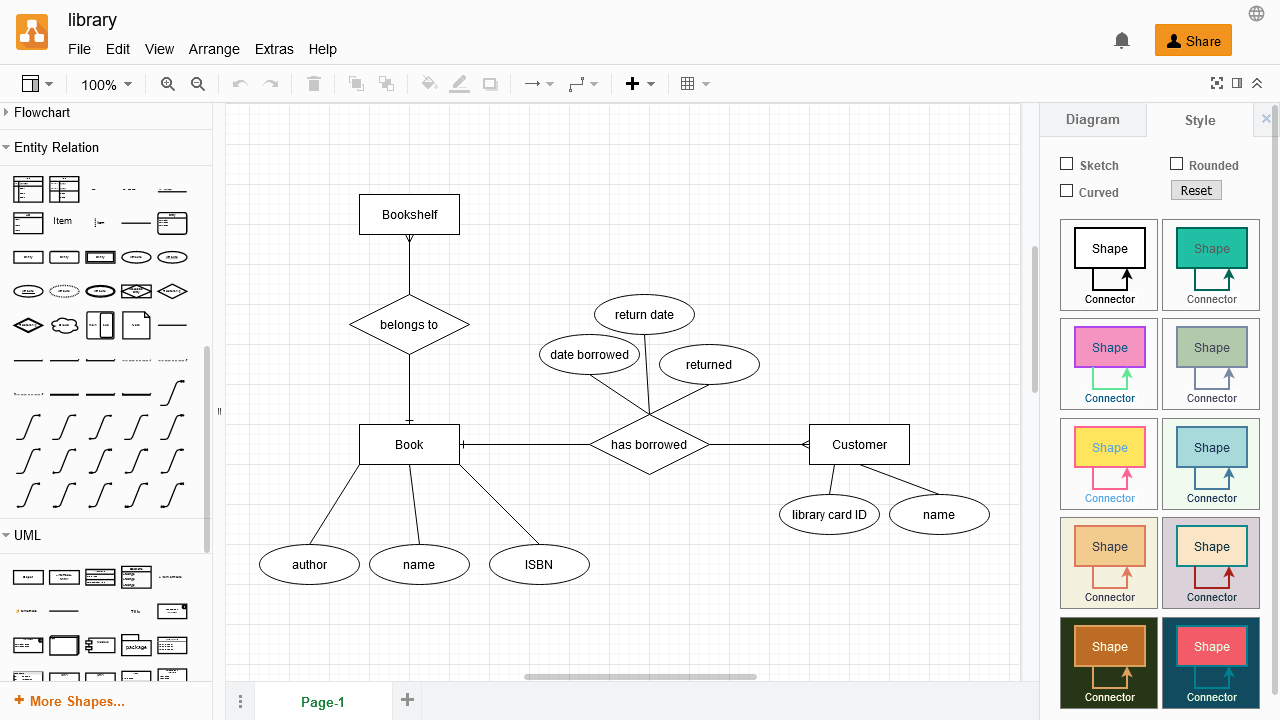
\includegraphics[width=\textwidth]{../img/diagrams.net.png}
  \caption{Tvorba ER diagramu v aplikaci diagrams.net}
  \label{fig:diagrams.net}
\end{figure}

\section{drawSQL}

Srovnávací kritéria:
\begin{itemize}
  \item kategorie -- logická vrstva,
  \item typ úložiště -- online, poskytované autory produktu
  \item export -- schématický (obecný SQL i platformě specifické formáty),
  rastrový PNG, serializovaný (JSON, v době psaní práce se chystá)
  \item živá spolupráce -- pouze v placené verzi,
  \item komercializace -- omezená verze navždy zdarma, různé měsíčně placené
  plány.
\end{itemize}

drawSQL je modelovací nástroj pro tvorbu relačních schémat. Aplikace je dostupná
ve webovém prohlížeči na adrese \url{https://drawsql.app}. Je vyvinuta ve
standardních webových technologiích a používá framework Vue.js. Plán zdarma
umožňuje tvorbu veřejně přístupných diagramů, které mohou mít maximálně 15
tabulek (entit). Měsíčně placené plány umožňují vytvářet neveřejné diagramy,
více (až nekonečně mnoho) tabulek v diagramu, více uživatelů, kteří mohou na
diagramu spolupracovat a přístup k verzovacím nástrojům. K vyzkoušení i
používání nástroje je potřeba uživatelský účet.

Hlavní funkcí drawSQL je export schématu do SQL. Proto si uživatel při vytváření
diagramu zvolí cílovou databázi, pro kterou schéma tvoří. Výsledné SQL tak bude
mít tvar, se kterou cílová databáze umí pracovat. Podporovanými databázemi jsou
MySQL, PostgreSQL a SQL Server.

Rozhraní, které je vidět na obrázku \ref{fig:drawsql}, obsahuje diagram a
postranní panel. V postranním panelu lze vytvářet jednotlivé tabulky, definovat
jejich sloupce a vlastnosti jednotlivých sloupců -- typ sloupce, nullability,
zda se jedná o primární klíč, unikátní klíč nebo index. Tyto změny se v reálném
čase reflektují v diagramu, ve kterém může uživatel jednotlivé sloupce spojovat,
čímž vytváří cizí klíče. Pozici těchto lomených čar lze upravovat pouze
posunutím tabulky v diagramu. Pokud je cizích klíčů víc, začne být diagram velmi
nepřehledný.

Diagram lze importovat ze souboru SQL stisknutím File $\rightarrow$ Import.
Stisknutím tlačítka File $\rightarrow$ Export se otevře nabídka Export, ve které
může uživatel diagram exportovat do SQL své předem zvolené databáze, nebo do
rastrového obrázku ve formátu PNG. Vývojáři aplikace plánují implementovat také
export diagramu pomocí serializace do formátu JSON. V nabídce Export je navíc
možnost nechat si vygenerovat platformně specifický kód jako například migrační
třídy pro Laravel, definice modelů pro Laravel a migrační schémata pro AdonisJS.

Živá spolupráce je k dispozici pouze v placené verzi. Dle našeho názoru je živá
spolupráce hlavní funkcí tohoto nástroje oproti konkurenčním relačním
modelovacím nástrojům. Některá integrovaná vývojová prostředí (např. Visual
Studio) obsahují nástroj pro relační modelování i generování databázového
schématu. Hlavním omezením těchto nástrojů je však absence živé spolupráce,
jedná se spíše o spolupráci iterací. Proto považujeme určení živé spolupráce za
placenou funkci za negativní rozhodnutí pro využitelnost nástroje v relaci s
konkurencí.

drawSQL také zveřejňuje šablony modelů (jedná se spíše o příklady) na adrese
\url{https://drawsql.app/templates}. Šablony jsou většinou potenciální modely
známých produktů (např. WordPress) a tvoří je autoři drawSQL. Tuto funkci
považujeme za výhodu, protože společnosti a individuální vývojáři se mohou
inspirovat existujícími a ověřenými řešeními, případně nezačínat se svým modelem
od nuly.

Závěrem určíme výhody drawSQL:
\begin{itemize}
  \item příjemné uživatelské rozhraní (viz obrázek \ref{fig:drawsql}),
  \item možnost určení typu relace, o sémantiku se aplikace stará sama
  (one-to-one, one-to-many, many-to-many),
  \item několik platformě specifických generátorů modelu,
  \item šablony a příklady existujících modelů
\end{itemize}
a nevýhody:
\begin{itemize}
  \item nelze upravit ani přesunout lomené čáry spojující cizí klíče, což
  způsobuje chaos pokud je v diagramu větší množství entit,
  \item živá spolupráce pouze v placeném plánu,
  \item správa verzí pouze v placeném plánu,
  \item k vyzkoušení nástroje je potřeba uživatelský účet,
  \item podporuje pouze relační databáze.
\end{itemize}

\begin{figure}
  \centering
  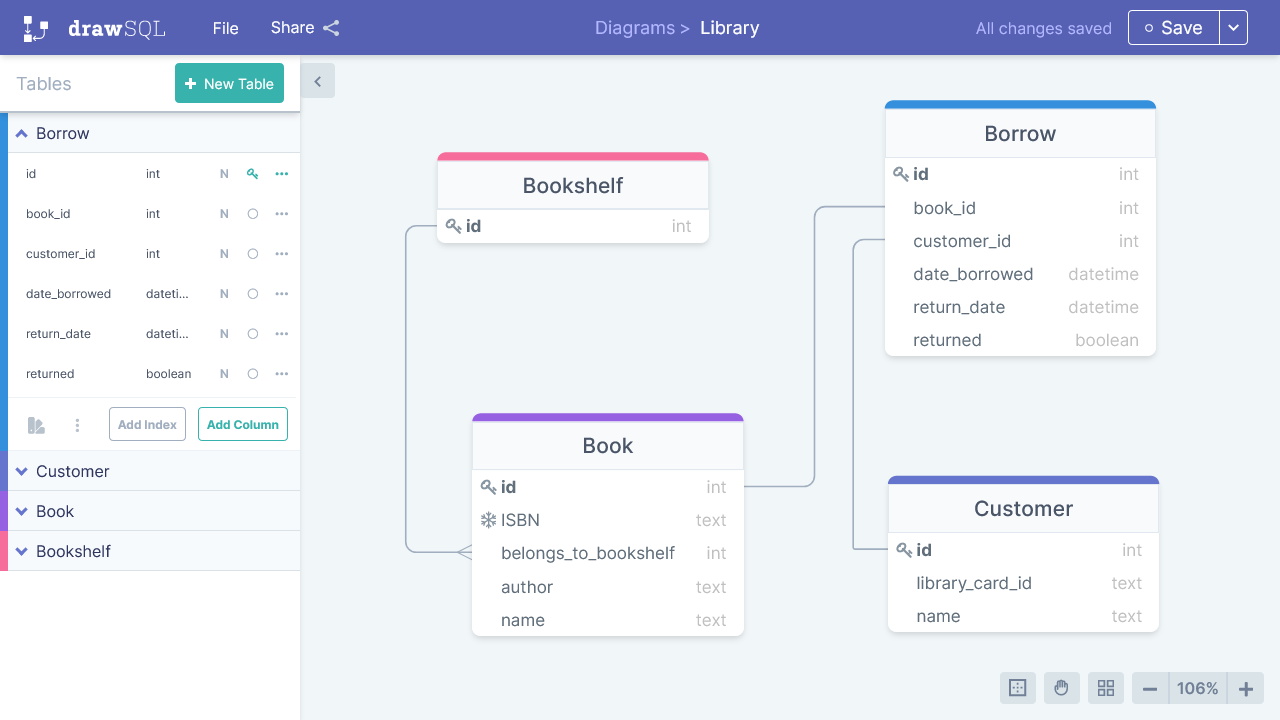
\includegraphics[width=\textwidth]{../img/drawsql.png}
  \caption{Tvorba diagramu v drawSQL}
  \label{fig:drawsql}
\end{figure}

\section{ERDPlus}

ERDPlus je modelovací nástroj pro tvorbu ER diagramů, relačních schémat a
hvězdicových schémat. Aplikace je dostupná ve webovém prohlížeči na adrese
\url{erdplus.com}. Její uživatelské rozhraní je tedy vyvinuto ve standardních
webových technologiích -- HTML, CSS a JavaScript -- a dále využívá framework
React pro tvorbu rozhraní v jazyce JavaScript.

ERDPlus lze používat bez založení uživatelského účtu a vytvořený diagram
exportovat do speciálního formátu erdplus, nicméně uživatel tak přijde o možnost
využití úložiště diagramů na serveru aplikace. Služby ERDPlus nejsou žádným
způsobem zpoplatněny.

Tvorba ER diagramů je intuitivní s jednoduchým uživatelským rozhraním, které je
vidět na obrázku \ref{fig:erdplus}. Uživatel má na výběr mezi vytvořením entity,
atributu, relace, spojení mezi těmito objekty a jednoduchého textového popisku.
V pravé části rozhraní se nachází panel s vlastnostmi zvoleného objektu. V tomto
panelu může uživatel také rychleji tvořit atributy entit a relací. Při zvolení
relace lze v panelu zvolit entity, které mají být v relaci, a spojení je pak
automaticky vytvořeno. Zároveň lze zvolit jednotlivé multiplicity relace.

ER diagram lze exportovat do rastrového formátu PNG. Zajímavou funkcí je také
převod do relačního schématu. Tato funkce je dostupná pouze tehdy, když uživatel
ER diagram uloží na server ERDPlus. Poté zvolí možnost \emph{Convert to
Relational Schema} a ERDPlus vytvoří nové relační schéma. Z relačních schémat
lze podobně vygenerovat SQL.

\begin{figure}
  \centering
  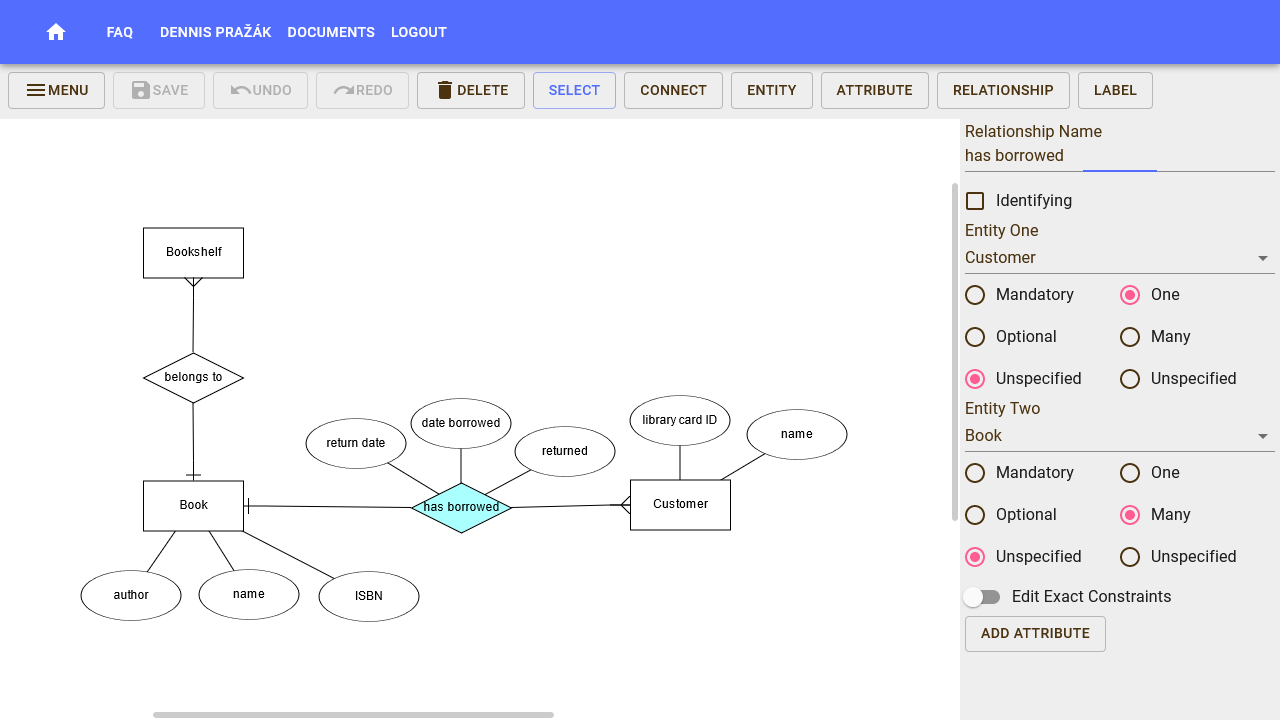
\includegraphics[width=\textwidth]{../img/erdplus.png}
  \caption{Tvorba ER diagramu v ERDplus}
  \label{fig:erdplus}
\end{figure}
\newcommand{\tnote}[1]{\textsuperscript{#1}}
\begin{table}
  \begin{center}
    \begin{tabular}{r|ccc}
      \toprule
      název produktu    & \textbf{diagrams.net}  & \textbf{drawSQL} & \textbf{ERDPlus} \\
      \midrule
      kategorie (vrstva)& libovolné diagramy & logická & konceptuální \\
      serializovaný export & \cmark & \xmark\tnote{\ref{tab:ec:plan}} & ? \\
      rastrový export   & \cmark        & \cmark  & \cmark  \\
      vektorový export  & \cmark        & \xmark  & \xmark \\
      schématický export (SQL) & \xmark & \cmark & \cmark \\
      zjednodušený export & ? & ? & ? \\
      poskytuje úložiště  & \xmark\tnote{\ref{tab:ec:external-storage}} & \cmark  & \cmark  \\
      využívá paměť prohlížeče & \cmark & &  \\
      \midrule[\heavyrulewidth]
      \end{tabular}
  \end{center}
  
  \footnotesize
  \begin{enumerate}[a.,ref=\alph*,noitemsep]
    \item plánovaná funkce \label{tab:ec:plan}
    \item využívá úložiště třetích stran \label{tab:ec:external-storage}
  \end{enumerate}
  
  \caption{Srovnání existujících řešení}
  \label{tab:existing-comparison}
\end{table}